\section{Results}

Partition Examples: Without any partitioning operation, the inner and outer boundary of of a shell model needs to be filled by a huge amount of support materials in order to guarantee a fine surface quality. See Figure \ref{fig:dear-simulation} (a-b) for an illustration of a deer model, both its inner and outer surface requires some amount of support in order not to be collapsed during the printing process; while our approach only keeps all cylinder-like shells that are free of support (Figure \ref{fig:dear-simulation} (c-d)).

\begin{figure}[tbp]
  \centering
  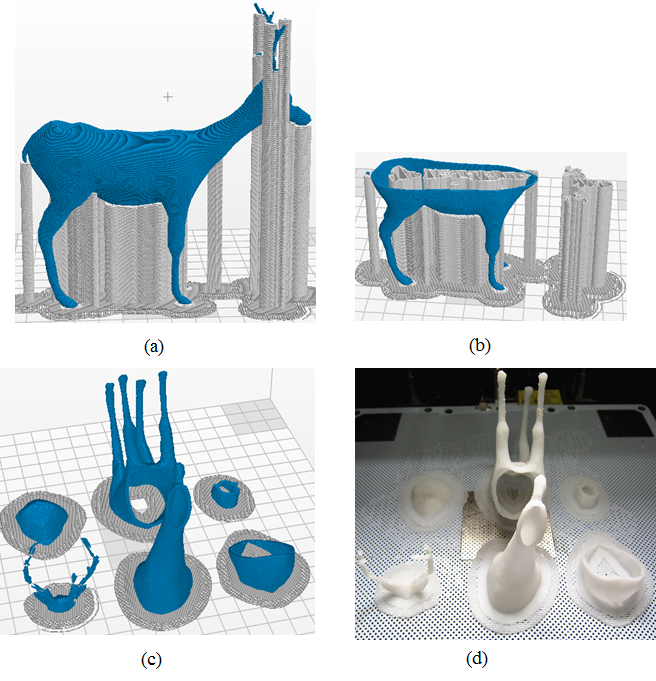
\includegraphics[width=\linewidth]{figs/dear-simulation.png}
  \caption{\label{fig:dear-simulation}%
           An illustration of a deer model under the 3D printing software Z-suite as the support angle is no larger than $20^{\circ}$; (a) the full model; (b) an intermediate step of the simulation; (c) the simulation result of our partitioned shell models; (d) the 3D printed shell models free of support.}
\end{figure}

We have run our algorithm on various natural or man-made models, and some of the results are presented as follows:

\begin{figure}[tbp]
  \centering
  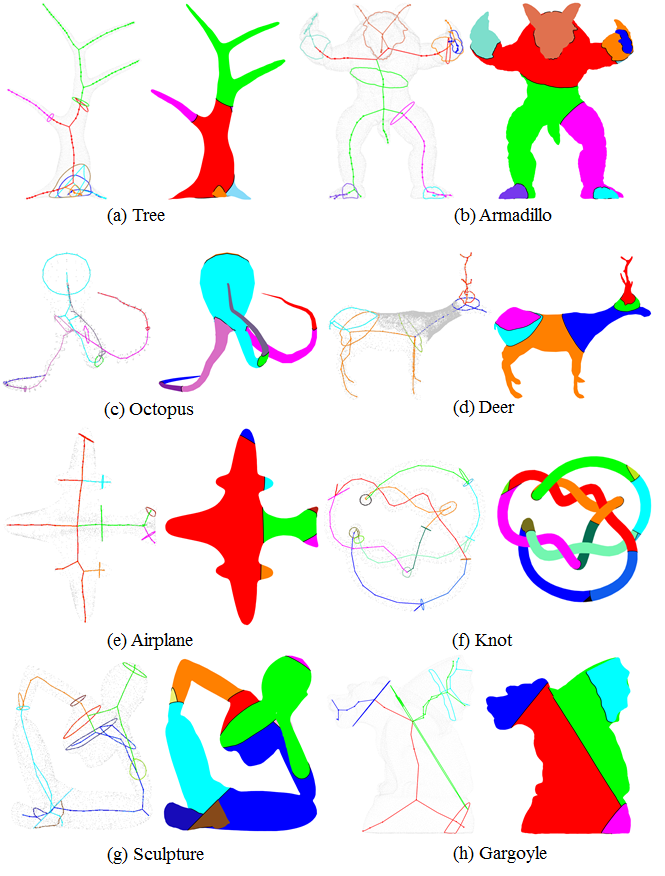
\includegraphics[width=0.45\textwidth]{figs/programming.png}
  \caption{\label{fig:programming}%
           Partition examples as $\theta = 70^{\circ}$. The printing direction of each part is orthogonal to its base (shown in the same color as the part)}
\end{figure}

Experimental Validation: We validated our approach by a set of printing experiments on Zortrax desktop printer, a kind of FDM machine that allows a printing layer thickness of 0.09mm , this is also the layer thickness we used in the printing experiments. The experiments are based on the choice of $\theta = 70^{\circ}$, i.e., all overhangs with an angle of no larger than $20^{\circ}$ with respect to the build platform are given support structures. Zortrax provides a built-in 3D printing software called \emph{Z-suite} can automatically counts the filament of the print material (in meters) and an estimate of the weight of the print material. The following table summarizes the printing material and time costs by the original models and the partitioned models. Our proposed skeleton-based partitioned approach reduce both the printing material and time significantly because the partition reduce both the supported materials inside and outside the models.



\begin{table*}[htb]

\begin{footnotesize}

\begin{center}

    \begin{tabular}{ p{1cm} p{1.5cm} p{1.5cm} p{1.81cm} p{1.53cm} p{1.5cm} p{1.7cm} p{1.7cm} }

    \hline

     Models& Print material (original)& Print time (original)& Number of parts (partition)& Print material (partition)& Print time (partition)& Material save (\%) &Time save(\%)\\ \hline
     Tree& 9.07m (22g)& 5h 5min & 8 &5.19(12g) & 4h 2min & 42.7784 &20.6557\\ \hline
     Armadillo& 9.85m (23g)& 5h 56min & 10  &4.65(11g) & 3h 30min & 52.7919 &41.0112\\ \hline
     Octopus& 14.58m (35g)& 8h 7min & 9  &8.75(21g) &6h 51min & 39.9863 &15.6057\\ \hline
     Deer& 14.24m (34g)& 8h 46min & 6  &8.89(21g) &5h 25min & 37.5702 &38.2129\\ \hline
     Airplane& 9.86m (23g)& 4h 15min & 7 &5.24(12g) &3h 10min & 46.856 &25.4902\\ \hline
     Knots& 26.96m (64g)& 17h 44min & 15 &12.38(29g) &11h 20min & 54.0801 &36.0902\\ \hline
     Sculpture& 28.21m (67g)& 14h 36min & 10 &11.62(28g) &10h 0min & 58.8089 &31.5068\\ \hline
     Gargoyle& 7.88m (19g)& 4h 34min & 5 &5.16(12g) &3h 48min & 34.5178 &16.79\\ \hline

  \hline

    \end{tabular}

\end{center}

\end{footnotesize}

\caption{Statistics showing the print material, print time and partition number of the printed models.}\label{tab:ertms:summary}

\end{table*}



Figure \ref{fig:experiment} shows the comparison of the printing effects of the original models and our partitioned models.

\begin{figure}[tbp]
  \centering
  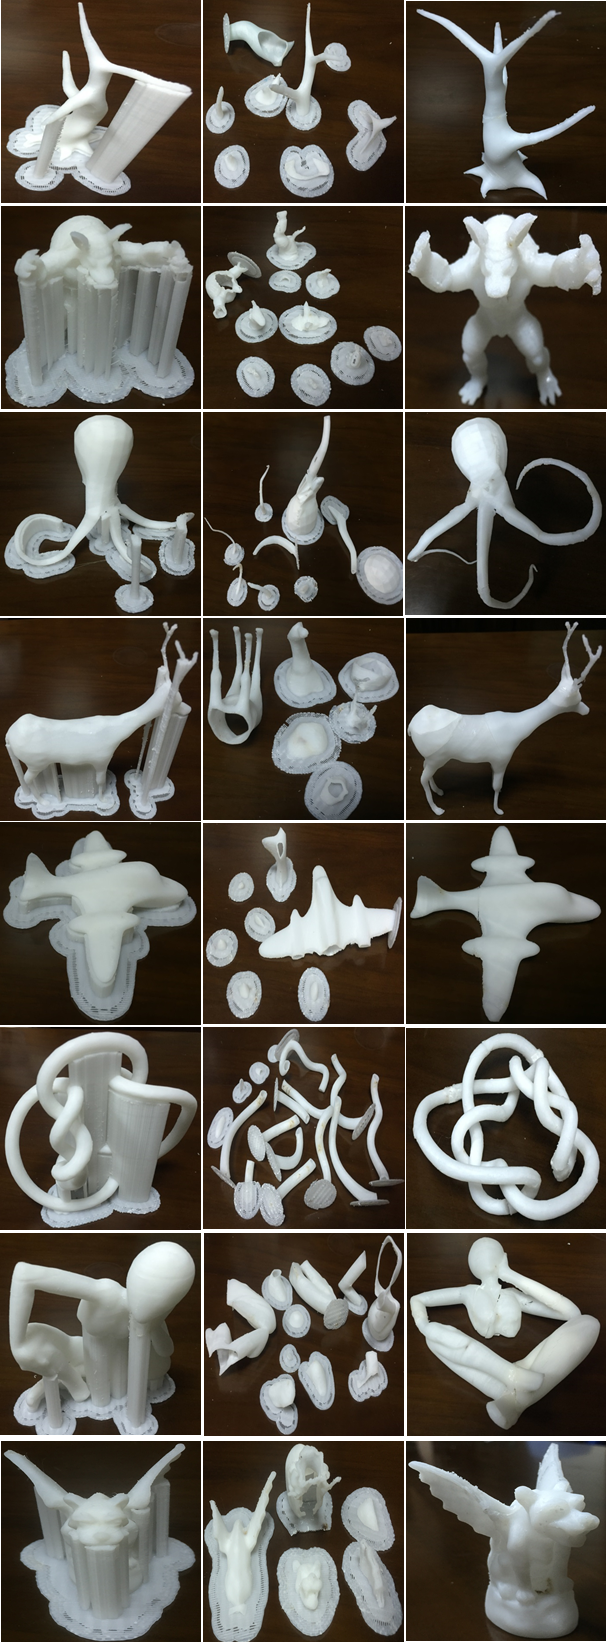
\includegraphics[width=0.48\textwidth]{figs/experiment.png}
  \caption{\label{fig:experiment}%
           A comparison between printing of original shell models and our partitioned models.}
\end{figure}


Although the FDM printing technique requires a small supporting bed for holding the printed model on the printing platform, other printing techniques such as SLA, SLM and SLS may avoid the use of these supporting beds. Therefore, our approach guarantees support-free to the most extent for all exiting printing techniques.

\hl {[Evaluations: how close we are to the global optimum][Limitations: discussion about 1. the strength of our interior, -- future work. 2. cut through salient regions -- hard to balance. etc]}

Since the problem of partitioning the skeleton graph into the least number of support-free subgraphs is NP-hard, it is impossible to obtain an optimal result in polynomial time. However, we can evaluate the effectiveness of our approach by judging the topology of some simple models and evaluate how close our partition is far away from a potential optimal result. For example, from Figure \ref{fig:ex1}, under the requirement of $\theta = 70^{\circ}$, ignoring the tinny detail geometric features we can roughly judge that the deer model requires at least 4 cuts: the tail, the chunk including the legs, the neck, and the head and the horn. Our approach provides a partition of 4 cuts, which is almost near the optimal. Further, from the appearance of the gargoyle model (the last row of Figure \ref{fig:experiment}), we can see that an optimal cutting should have the following 4 parts: the head, two wings, and the remaining parts. Our partition results in 5 parts, which is very close to the potential optimal partition.

Our approach is devoted to shell models, it can also be applied to cutting solid models without any problem. However, our approach suffers from a few limitations: for shell models, the thickness of the shells need to be large enough such that no serious deformation is caused during the assembling process. However, the problem of setting the minimum thickness of the model for various parts of the model is a challenging problem, and our current work is restricted to a uniform setting of the shell thickness whose value is determined by an error-and-trial process. Further, the strength guarantee is not elaborated in this work, a possible solution is to use the algorithm in \cite{WangWYLTTDCL13} that distributes the least amount of materials for constructing a truss frame beneath the skin. Finally, our approach may allow a cut that passes through a salience region, which may hurt the appearance of the model. But it is very difficult to make a balance between the two since out cuts are flat. A potential future research is to take care of salience region while making cuts. Finally, as a trade-off, if a spatially curved cut is allowed, then the salience regions can be preserved properly.
